
\section{Testing}
\thispagestyle{plain}
System testing or software testing, falls into something that is called “Black-box testing”. This is a method of software testing, that investigates the functionality of the application. Eg. what it does, it is simply described as this:
It will not require to know how to code, or need any sufficient level of skill to programming when an system test is about to go down. It will neither interfere with it’s internal structure or workings. 

\subsection{Testing Procedure}

When you are about to conduct a test, you find a test-person. Then you tell them what the software is supposed to do. And give them the Test cases[7.2], and explain to them it is very important to think loud so we get the most out of the testing. 

\subsection{Test Cases}

Test cases are built around the specifications and requirements of the application. What the application is supposed to do.  

\begin{table}[htp]
\begin{center}
\begin{tabular}{ i{4cm} ||  i{10cm}} \toprule
\multicolumn{2}{c}{\textbf{Get Places}} \\ \hline
ID & T-F1 \\ \hline
Requirements & SF-1 \\ \hline
Feature& Places are shown on the map \\ \hline
Preconditions& \begin{enumerate} \item Flickr is up \item The Flickr group contains photos with locations \item Application is installed on device \item Device is connected to the internet \end{enumerate} \\ \hline
Test Description& \begin{enumerate} \item Open the application \item Wait for 30 seconds \item Click on a pinpoint \item Zoom out to a world view  \end{enumerate} \\ \hline
Expected result & The map should show some clickable pinpoints. When clicked the pinpoints should open a little box containing a thumbnail picture and small text provided by the Flickr Stedr group. \newline
When zoomed out new places should be loaded according to what the user see. \\ \hline
Pass/Fail criteria & The test is considered a pass if the expected result happens. The last step that need to be passed is that the place at Grenada is shown. \newline
If there are any incosistencies with the expected result, the test should be considered a fail. \\ \hline
Severity & High\\ \bottomrule
\end{tabular}
\end{center}
\caption{Test Case: Get Places}
\label{tab:Test Case: Get Places}
\end{table}


\begin{table}[htp]
\begin{center}
\begin{tabular}{ i{4cm} ||  i{10cm}} \toprule
\multicolumn{2}{c}{\textbf{Open menu}} \\ \hline
ID & T-F2 \\ \hline
Requirements & SF-2 \\ \hline
Feature& Drawer menu with options is opened. \\ \hline
Preconditions& \begin{enumerate} \item[ ]1,2,3,4 \end{enumerate} \\ \hline
Test Description& \begin{enumerate} \item Click on the menu button \item Click on all of the icons in the menu \item Click on the menu again \end{enumerate} \\ \hline
Expected result & When the menu button is pressed, a drawer menu should open. All of the icons in the drawer menu is also buttons and when clicked again, the menu button should close the drawer menu. \\ \hline
Pass/Fail criteria & The test is considered a pass if the menu button opens and closes a drawer menu. Also, all of the icons should \\ \hline
Severity & High\\ \bottomrule
\end{tabular}
\end{center}
\caption{Test Case: Open Menu}
\label{tab:Test Case: Open Menu}
\end{table}


\begin{table}[htp]
\begin{center}
\begin{tabular}{ i{4cm} ||  i{10cm}} \toprule
\multicolumn{2}{c}{\textbf{Views}} \\ \hline
ID & T-F3 \\ \hline
Requirements & SF-6 \\ \hline
Feature& All the views are accessible \\ \hline
Preconditions& \begin{enumerate} \item[ ]1,2,3,4 \item[T-F1] Get places \end{enumerate} \\ \hline
Test Description& \begin{enumerate} \item Click on a pinpoint \item Click on the small window that appears \item Click on one of the buttons \textit{Images, Sound, Story} \item Dependent on the prevoius step, click on the buttons not yet pushed \item Click the menu button \item Click home \end{enumerate} \\ \hline
Expected result & Which view that is selected is shown to the user by being in a different color than the two other buttons. If the button for the selected view is touched, nothing should happen. \newline
 For every button representing a non-selected view, the user should be taken to the view as indicated by the button text. \\ \hline
Pass/Fail criteria &The test is passed if the button: \newline[5pt]
Image - Takes you to the image view\newline
Story - Takes you to the story view\newline
Sound - Takes you to the sound view.\newline[5pt]
The selected view has a unclickable button in a different color representing the selected view.\newline
Considered a fail if there are any inconsistencies with the criterias above. \\ \hline
Severity & High\\ \bottomrule
\end{tabular}
\end{center}
\caption{Test Case:  Views}
\label{tab:Test Case: Views}
\end{table}


\begin{table}[htp]
\begin{center}
\begin{tabular}{ i{4cm} ||  i{10cm}} \toprule
\multicolumn{2}{c}{\textbf{Load Content}} \\ \hline
ID & T-F4 \\ \hline
Requirements & SF-7 \\ \hline
Feature& Content is loaded for the places \\ \hline
Preconditions& \begin{enumerate} \item[T-F3] Views \end{enumerate} \\ \hline
Test Description& \begin{enumerate} \item Click on a pinpoint(not Camera Obscura) \item Click on the description \item Go through the views as in T-F3 \item[3a] Click on all of the titles on the story \item[3b] Click on two random images \item[3c] Click on a sound \end{enumerate} \\ \hline
Expected result &The places should be loaded with relevant and accessible content from all of the content providers.. \newline
If some content-types aren’t provided for the specific place, the content type should be loaded but indicate that it is empty. \\ \hline
Pass/Fail criteria &The test is considered a pass if the expected result happens. \newline
If there are any inconsistencies with the expected result, the test should be considered a fail. \\ \hline
Severity & High\\ \bottomrule
\end{tabular}
\end{center}
\caption{Test Case: Load Content}
\label{tab:Test Case: Load Content}
\end{table}



\begin{table}[htp]
\begin{center}
\begin{tabular}{ i{4cm} ||  i{10cm}} \toprule
\multicolumn{2}{c}{\textbf{Collection view}} \\ \hline
ID & T-F5 \\ \hline
Requirements & SF-8 \\ \hline
Feature& Show a view with the stories related to a collection \\ \hline
Preconditions& \begin{enumerate} \item[T-F2] Open menu \item[T-F4] Load Content \item[5] It exist a collection \end{enumerate} \\ \hline
Test Description& \begin{enumerate} \item Press the menu button \item Press the Collection button \item Press a collection \end{enumerate} \\ \hline
Expected result & When the collection button is pressed a new view should open with the list of stories related to the collection. \\ \hline
Pass/Fail criteria & The test is considered a pass if it is possible to open the menu and access a collection with a list of stories. \\ \hline
Severity & Medium\\ \bottomrule
\end{tabular}
\end{center}
\caption{Test Case: Collection View}
\label{tab:Test Case: Collection View}
\end{table}


\begin{table}[htp]
\begin{center}
\begin{tabular}{ i{4cm} ||  i{10cm}} \toprule
\multicolumn{2}{c}{\textbf{Collection map view}} \\ \hline
ID & T-F6 \\ \hline
Requirements & SF-8 \\ \hline
Feature& Show places related to a collection as pinpoints in a map \\ \hline
Preconditions& \begin{enumerate} \item[T-F2] Collection View \end{enumerate} \\ \hline
Test Description& \begin{enumerate} \item Press the menu button \item Press the Collection button \item Press a collection \item Press the \textit{show on map}-button \end{enumerate} \\ \hline
Expected result &When the “show on map”-button is clicked, a map view should open with related places showed as pinpoints. Pinpoints not related to the collection should not be placed on the map. \\ \hline
Pass/Fail criteria & The test is considered a pass if all places related to a collection is exclusively shown in a map view. \\ \hline
Severity & Medium\\ \bottomrule
\end{tabular}
\end{center}
\caption{Test Case: Collect Map View}
\label{tab:Test Case: Collect Map View}
\end{table}


\begin{table}[htp]
\begin{center}
\begin{tabular}{ i{4cm} ||  i{10cm}} \toprule
\multicolumn{2}{c}{\textbf{Gallery}} \\ \hline
ID & T-F7 \\ \hline
Requirements &  \\ \hline
Feature& Gallery function\\ \hline
Preconditions& \begin{enumerate} \item[T-F4] Load Content \item[ ] The application is in aplcae with a story where there are multiple images to the story. \end{enumerate} \\ \hline
Test Description& \begin{enumerate} \item Press the story title \item If there are more pictures related to a story, press the arrows \end{enumerate} \\ \hline
Expected result &When accessing stories with multiple pictures as content, arrows indicating the possibility to go through picture files should appear. When pressed new images should replace the old picture. \\ \hline
Pass/Fail criteria &The test is considered a pass if the expected result happens. \newline
If there are any inconsistencies with the expected result, the test should be considered a fail. \\ \hline
Severity & Low\\ \bottomrule
\end{tabular}
\end{center}
\caption{Test Case: Gallery}
\label{tab:Test Case: Gallery}
\end{table}


\begin{table}[htp]
\begin{center}
\begin{tabular}{ i{4cm} ||  i{10cm}} \toprule
\multicolumn{2}{c}{\textbf{Upload Content}} \\ \hline
ID & T-F8 \\ \hline
Requirements &  SF-9\\ \hline
Feature& Content can be uploaded to Instagram, Twitter and SoundCloud \\ \hline
Preconditions& \begin{enumerate} \item[T-F4] Load Content \item[6] Successfully connected to the content (not story provider) providers \end{enumerate} \\ \hline
Test Description& \begin{enumerate} \item Click on a pinpoint \item Click on the description \item Go through the views as in T-F3 \item Upload textual content to Twitter \item Upload picture to Instagram \item Upload sound to SoundCloud \end{enumerate} \\ \hline
Expected result &The places should be loaded with relevant and accessible content from all of the content providers..\newline
If some content-types aren’t provided for the specific place, the content type should be loaded but indicate that it is empty. \\ \hline
Pass/Fail criteria & The test is considered a pass if the expected result happens. \newline
If there are any inconsistencies with the expected result, the test should be considered a fail. \\ \hline
Severity & Medium\\ \bottomrule
\end{tabular}
\end{center}
\caption{Test Case: Upload Content}
\label{tab:Test Case: Upload Content}
\end{table}

\clearpage

\subsection{Test Execution}
\subsubsection{Acceptance Testing}
Acceptance testing is one of the last levels of the software testing process. The purpose of such testing is to evaluate the system's compliance with the given requirements to check wether is is acceptable for delivery. Hence the name accepance testing.

On may 14. during one of our last meetings we sat down with Jaqueline Floch for the final acceptace test of our system. Since the project has been more based on furter developing features than improving the graphical user interface and increasing usability, we had a more feature based acceptance testing where we went through the requirement list. Not to say that usability is not as important, but in addition to have had less focus than the new features, our customer have recieved the latest build almost every week in the later stages of the project. Through this, the customer have conducted something similar to a usability based acceptance test regurlary throughout the project, to which we recieved feedback \todo{(Examples of feedback can be found in Appendix X)}. Based on this we found usability based user acceptance test, which we know is the way many of the other groups have chosen to handle the test, to be redundant.
The test was conducted by going through the requirement list sorted by priority and individually recieving a verdict on acceptance. The individual requirement either revieved \texttt{Pass, fail, outdated} or \texttt{cancel} if the requirement was pulled. The latter was the case on a lot of the requirements with lower priotity since we had little time and the customer wanted us to focus on the more important tasks.

The result of the acceptance test are listed below:\\

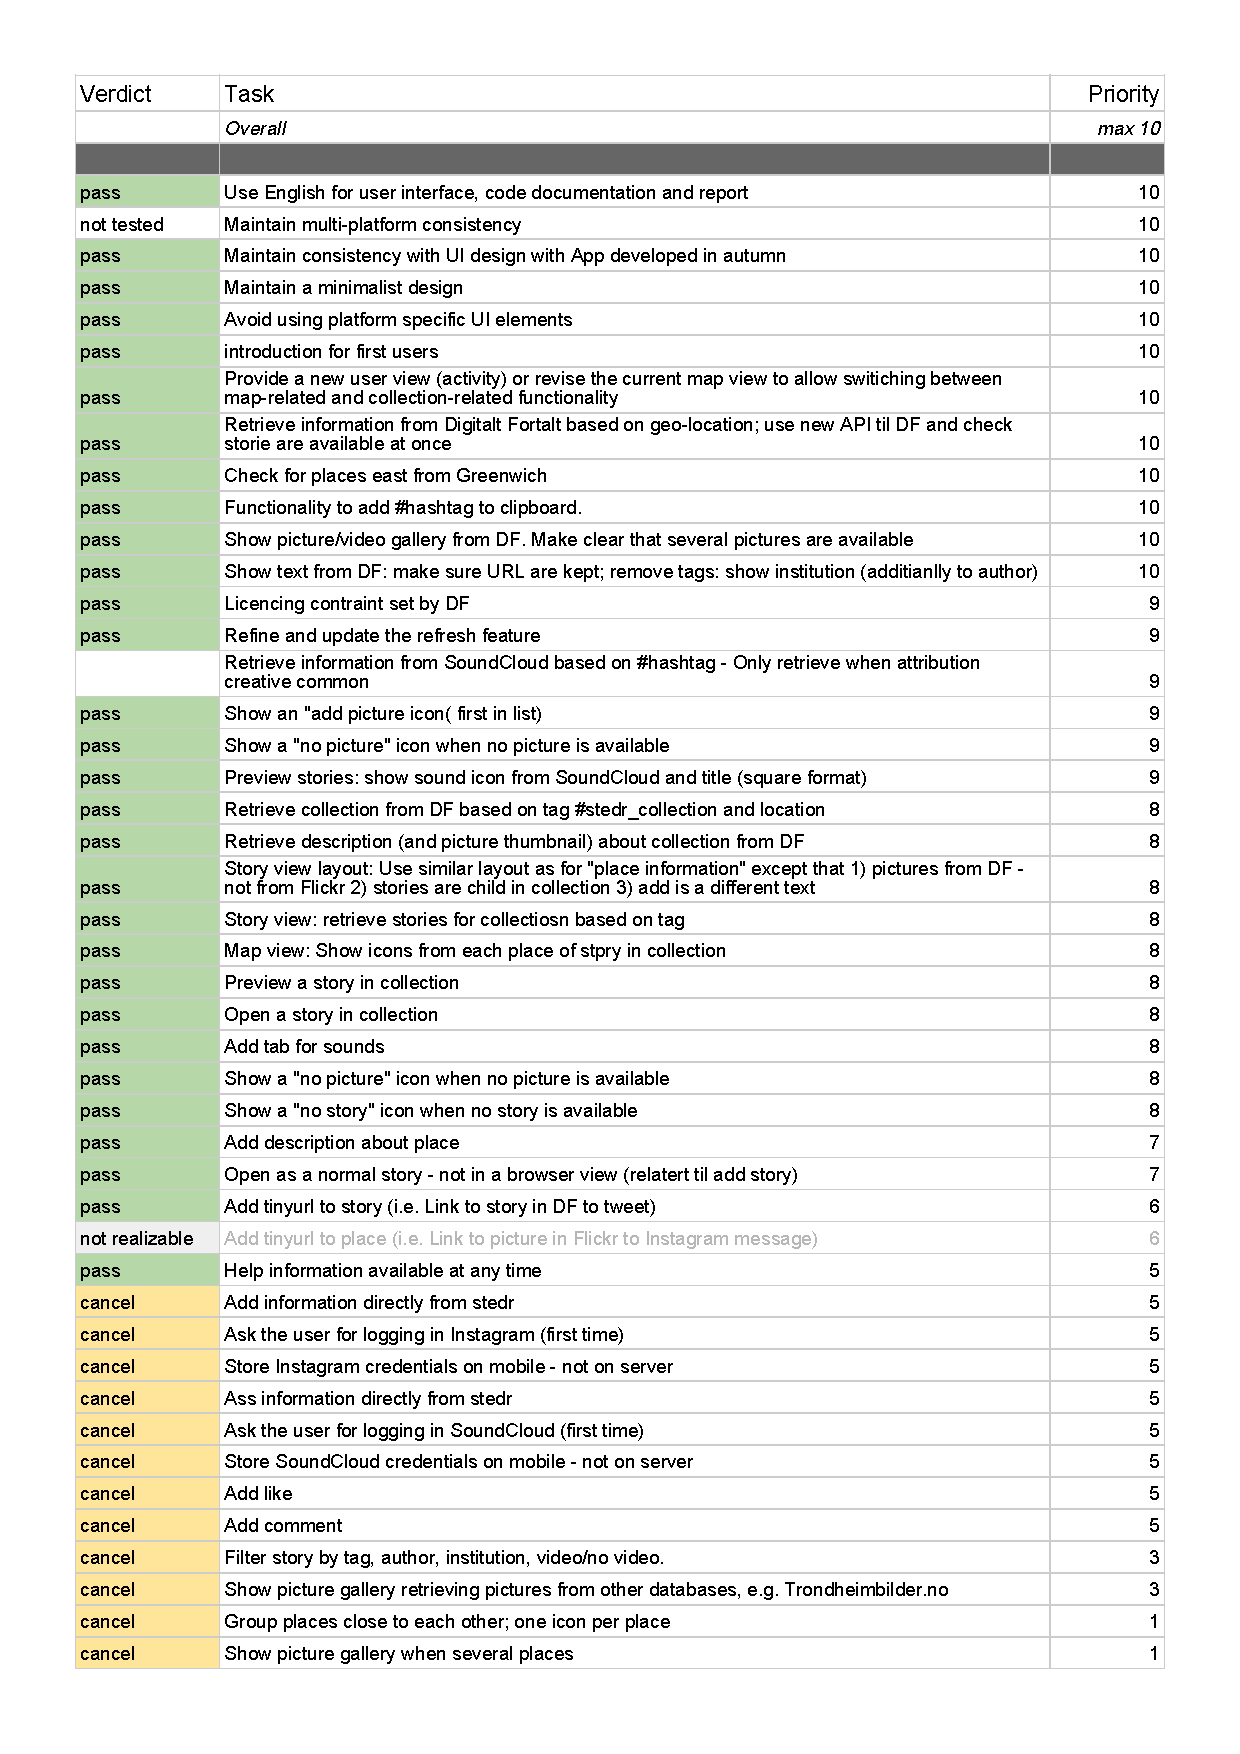
\includepdf[%
 	pages={-},
	offset=0in 0in,%
	addtolist={%
		\thepage, table, {Acceptance Testing}, tab:AcceptanceTest
	},
	]{res/AcceptanceTesting_Requirements.pdf}

\subsubsection{NFR testing}
It is important for the project that our result meets the projects main non-functional requirements, described in the ``Product quality'' section of the SRS chapter \todo{chapter 4.12}, for it to be considered a success. 

\paragraph{Compability}

\paragraph{Performance Efficiency}
We have greatly improved the core of the system to boost the efficiency of the application, this should cause the application to use no more than 300 seconds to pull new content from the APIs. The efficiency was tested by adding new content and recording 10 times with different content posted at different times. By measuring the individual response times and calculating the average result we will get a rough estimate.\\

\begin{table}[!htp]
\begin{center}
	\begin{tabular}{ | l | l | l | r | }
	\hline
	 \#	 	& Content 		& Time a day 		& Result \\ \hline
	 1		&Instagram		& 14:40			& \texttt{1 sec} \\ \hline
	 2		&Instagram		& 10:55			& \texttt{1 sec} \\ \hline
	 3		&Instagram		& 14:45			& \texttt{1 sec} \\ \hline
	 4		&Tweet		& 14:16			& \texttt{19 sec} \\ \hline
	 5		&Tweet		& 14:18			& \texttt{20 sec} \\ \hline
	 6		&Tweet		& 10:40			& \texttt{20 sec} \\ \hline
	 7		&Story		& 15:26			& \texttt{133 sec}\\ \hline
	 8		&Story		& 16:15			& \texttt{10 sec}\\ \hline
	 9		&Story 		& 11:00			& \texttt{104 sec}\\ \hline
	 10		&Story		& 15:48			& \texttt{135 sec}\\ \hline
	 11		&Story		& 16:03			& \texttt{107 sec}\\ \hline
	 12		&Story		& 19:01			& \texttt{132 sec}\\ 
	 \hline
 	 \end{tabular}
\end{center}
\caption{Performance Efficiency: Publishing New Content}
\label{tab:Performance Efficiency: Publishing New Content}
\end{table}

Since much of the test content had relatively consistent results we did not think more tests was needed. The Instagram images appeared almost instantly ( 1 second) consistently, since we completed the tests manualy, we could not measure finer times, something we thought was not needed due to the nature of the tests. The twitter content were a little slower as expected, but did also appear consistantly at a reasonable time averaging in just under 20 seconds. As for the stories we published through Digitalt Fortalt, the times were very inconsistent. In three of the tests (\# 7, \#10 and \#12), which was the longest ones, the content had to be uploaded to DF as well as being published, this probably added to the time. All the other tests were performed with the content already uploaded, just to be published, but we still recorded a massive swing in results ranging from \texttt{10 seconds} (\#8) to \texttt{105 seconds} (\#9).


Average: 
\begin{equation}
\frac{133 + 10 + 104 + 135 + 107 + 132}{6} = {103.5}
\end{equation}

With all results clocking in under 150 secons, and our goal being under 300 seconds, we are very pleased with the results and can happily see our app passing this test. Considering the version of the app we recieved sometimes needed multiple days for the results to appea, it is needless to say there have been a massive improvement.


Another important part of the performance efficiency are the application's data usage. Blowing the users' data limit and potentially taking a large part in increasing their phone-bill is something we want to avoid, and to avoid that we have implemented a data usage restraint. This restraint is set through the equation described in \todo{4.12.2}.

We tested the data usage to make sure our application met our standard. We measured this roaming unconnected to any wifi-hotspots while running the app.\\

\emph{Quick session}\\
Opening map: \texttt{55.74 kB}\\
Entering place with only one story: \texttt{+ 6.07 kB}

\emph{Browsing session}\\
Browsing map over Trondheim: \texttt{1.64 MB}\\
Entering place with 6 stories and 2 instagram pictures: \texttt{+ 0.02 MB}

We found these results to be pretty reasonable. The app does not download more content than necassary, and the results seems really consistent compared to the experiences we have had using the application.

\paragraph{Reliability}


\paragraph{Portability}

The multiplatform aspect of the project has played a major part in the development and have played a large part in our choice of environment and frameworks. What we want to achieve is a reasonable consistency through different platforms and versions. We have throughout the development process tested it with many different viritual devices on different settings, but the most valuable ones are the ones performed on the physical devices at our disposal.\\

\begin{table}[!htp]
\begin{center}
	\begin{tabular}{ | l | l | l | r | }
	\hline
	 \#	& Platform (version)	&Device			& Notes \\ \hline
	 1	&Android (4.4.2 KitKat)	&LG Nexus 5			& Works prefectly\\ \hline
	 2	&Android (4.3 Jelly Bean)	&Samsung Galaxy SII	& No notable differences or bugs\\ \hline
	 3&&&\\ \hline
	 4&&&\\ \hline
	 5&&&\\ \hline
	 6&&&\\ \hline
	 7&&&\\ \hline
	 8&&&\\ \hline
	 9&&&\\ \hline
	 10&&&\\ 
	 \hline
	 \end{tabular}
\end{center}
\caption{Portability Testing}
\label{tab:Portability Testing}
\end{table}


\/*

\subsubsection{Acceptance testing}



\begin{center}
\begin{tabular}{ i{4cm} ||  i{10cm}} \toprule
\multicolumn{2}{c}{\textbf{Select a place}} \\ \hline
Related test case (ID) & T-F1 \\ \hline
Test Description & We asked the user to open the app and browse the map to find a desired ``place''. \\ \hline
Steps & \begin{enumerate} \item Open the application \item Wait for response \item Browse the map and find a place of your choosing \item Select place by clicking on pinpoint \end{enumerate} \\ \hline
Result & The user had little issue doing the test, without hesitation or any questions, completeing the task with ease. The response we got was that the interface was very intuitive and that little effort was needed to understand how to proceed.  \\ \hline
Verdict & Passed \\ \bottomrule
\end{tabular}
\end{center}

*/

